\documentclass[12pt]{article}
%Gummi|065|=)
\usepackage{amsmath, amsfonts, amssymb}
\usepackage[margin=0.5in]{geometry}
\usepackage{xcolor}
%\usepackage{graphicx}
%\usepackage{graphicx}
\newcommand{\off}[1]{}
\DeclareMathSizes{20}{30}{21}{18}

\newcommand{\myhrule}{}

\newcommand{\dash}{
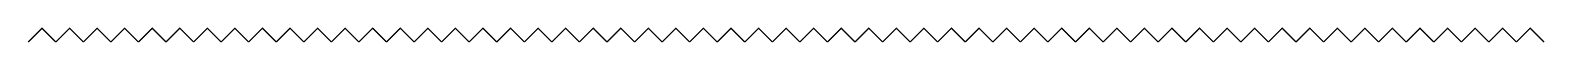
\begin{tikzpicture}[scale=0.35]
\foreach \x in {1,...,55}{
	\draw (\x,-0.25)--(\x+0.5,0.25)--(\x+1,-0.25);
}
\end{tikzpicture}
}

\usepackage{tikz}

\title{\textbf{ Examples:  Gamma Functions}}
\author{John D Mangual}
\date{}
\begin{document}

\fontfamily{qag}\selectfont \fontsize{25}{30}\selectfont

\maketitle

\noindent  I found this neat little formula on the internet:
$$ \frac{\Gamma(\frac{1}{24})\Gamma(\frac{11}{24})}
{\Gamma(\frac{5}{24})\Gamma(\frac{7}{24})}
= \sqrt{3} \cdot \sqrt{2 + \sqrt{3}} $$
My question was answered by Noam Elkies\footnote{Fellow Stuyesant alumnus} using various cheap multiplication tricks, he derives th formula in question.  He explains to me a bit what I am looking at, and why some of these equations might be happening.\footnote{Equations like these are divorced from applications.  I go to an engineer's desk and read one equation on page of his notes - completely irrelevant to the application he has in mind - and run with it.}\\ \\
The core equation: \textbf{mirror formula} is really kind of the only formula there is for the Gamma function:
$$ \Gamma(z) \Gamma(1-z) = \frac{\pi}{\sin \pi z}$$
\newpage

\noindent Given the connection between the Gamma function and the factorial: $\Gamma(n+1)=n!$ we get a relation between the factorial and the sine.\footnote{De Moivre's formula $ e^{ix} = \cos \theta + i \sin \theta $ is already quite exotic since it claims that exponentials and trigonometry are related.  More fudamentally:
$$ \textbf{size} \asymp \textbf{angle} $$ 
The relationship between factorial $n!$ and trig function $\sin \theta$ is a bit more exotic.} \\ \\
Here is one more:
$$ F( \tfrac{1}{4},\tfrac{1}{4};1;\tfrac{1}{64}) = \sqrt{\frac{2}{7\pi}} \times \left[\frac{ 
\Gamma(\frac{1}{7})\Gamma(\frac{2}{7})\Gamma(\frac{4}{7})
}{
\Gamma(\frac{3}{7})\Gamma(\frac{5}{7})\Gamma(\frac{6}{7})
}\right]^{1/2}$$
expressed in terms of the hypergeometric function.  I could not find an infinte product for general hypergeometric funtions, but there could be for special values.
$$F( \tfrac{1}{4},\tfrac{1}{4};1;\tfrac{1}{64})
= \frac{\Gamma(1)}{\Gamma(\frac{3}{4})\Gamma(\frac{1}{4})} \int_0^1  \frac{dz}{\sqrt[4]{z^3(1-z)(1-zx)}} $$
and $\Gamma(1) = 0! = 1!$ Just trying to make it look like binomial coefficients. \\ \\
In general there is something called \textbf{Chowla-Selberg} formula.  Legendre knew
$$ \int_0^{\frac{\pi}{2}} \frac{dt}{1 - k^2 \sin^2 t}
= \frac{2^{2/3} 3^{1/4}}{8\pi})\Gamma(\frac{1}{3})^3 $$
where $k = \sin \frac{\pi}{12}$ and there is an Elliptic curve related to $\mathbb{Q}(\sqrt{-3})$. \\ \\
And Elkies knew these special integrals are artifacts of possibly
\begin{itemize}
	\item  Colmez conjecture 
	\item  Abelian varieties or Shimura Varieties
	\item  Chowla-Selberg or Gross-Zagier formulas
	\item  Complex multiplication
	\item  Motives, Homology, etc
	\item  Andre-Oort conjecture
\end{itemize}
Unfortunately these are written in very complicated abstract language.   It is very likely that classical computations (with an $\int$-sign) could exhibit they phenomenon they are talking about. \\ \\
One shorthand they use is to say:
$$ \phi \in H^1 \longleftrightarrow \int_a^b  \in H^1   $$
I have written the correspondence in schematic and incorrect fashion.

\newpage

\noindent With zero knowledge of this field a few surprises already:
\begin{itemize}
	\item Why is there no special Gamma function for numberfields $\Gamma_{\mathbb{Q}(i)}$, $\Gamma_\mathbb{Q}(\sqrt{3})$? etc.
\end{itemize}
At the heart is the first contour integral we always know:
$$  \int_{-\infty}^\infty \frac{dx}{\sqrt{x^2 + 1}} = \tan^{-1} x \bigg|^\infty_{-\infty} = \frac{\pi}{2} - \bigg(-\frac{\pi}{2} \bigg) = \pi $$
There is lots of questions here.\footnote{ I just made up this formula I don't even remember -- I assume Cauchy residue formula is correct, without verifying the approximations made in the proof work.}  In between the lines this is a question about the curve:
$$ y^2 = x^2 + 1 $$
This is a hyperbola over real numbers $\mathbb{R}$, and is a \textbf{sphere} (genus 0) over $\mathbb{C}$. \\ \\ 
Here is the example from Colmez own paper.  Let $\epsilon = e^{i\pi/8}$ (this is an {\color{green!80!white}octogon})
$$ \int_\epsilon^{\epsilon^3} \frac{x^3 - x}{\sqrt{x^8 + 1}} \frac{dx}{x} = \frac{2\pi i}{8} (\epsilon^6 - \epsilon^2) \left( \frac{\Gamma(\frac{1}{2})}{
\Gamma(\frac{5}{8})\Gamma(\frac{7}{8})} \right)$$
Here it is instructive to draw the octogon where the poles should lie, and the line between two corners. 
\newpage

\noindent So what is this new-fangled language Math professors are talking about?  Here is a formula for a Faltings height:
$$ h_\text{Fal}( X_{y^2 = x^5 + 1})
= \log 2\pi - \frac{1}{2} \log \left(
\Gamma(\frac{1}{5})^5
\Gamma(\frac{2}{5})^3
\Gamma(\frac{3}{5})
\Gamma(\frac{1}{5})^{-1} \right) $$
Obviously this is an \textbf{entropy}.  Except I don't know what a Jacobian variety or a Faltings height.

\newpage

\noindent At least here are some of my own thoughts.  I might start by using Euler's formula for the factorial:
$$ \Gamma(x) = \lim_{n \to \infty} \frac{n^x n!}{x(x+1)(x+2)\dots (x+n)} $$
so what could we mean by re-ordering half an object?
$$\Gamma(\tfrac{1}{2}) = \lim_{n \to \infty}
\frac{ \sqrt{n} \;n!}{ \frac{1}{2} \times \frac{3}{2} \times \frac{5}{2} \times \dots \times \big(\frac{1}{2}+n\big)} $$
This number is related to the middle binomial coefficient.  We have that:
$$
\frac{1}{2} \times \frac{3}{2} \times \frac{5}{2} \times \dots \times \bigg( \frac{1}{2}+(n-1) \bigg)
= \frac{(2n)!}{2^n \, n!}
 $$
The DeMoivre-Laplace limit formula - for the middle binomial coefficient 
$$ \frac{(2n)!}{n! \times n!} =  \binom{2n}{n} \asymp
\; 2^{2n} \times \frac{1}{ \sqrt{\pi n}} $$
Somehow these stupid objects have to yield statements about Galois theory, L-functions, etc.
$$ \sin \pi x = \pi x\, \prod_{n \neq 0} \bigg(1 - \frac{x}{n}\bigg) $$
\newpage

\noindent Let's do an attempt at the modern language:
\Large
$$
\begin{array}{ccccc}
\frac{\zeta_E'(0)}{\zeta_E(0)} &=& \frac{1}{12h}\sum_{i=1}^h \log \big( \Delta(\mathfrak{a}_i)\big)
\Delta(\mathfrak{a}_i^{-1})\big)&=&-2h_{\text{Fal}}(X) + \frac{1}{2} \log D \\ 
\uparrow \downarrow & & & & || \\
\frac{\zeta'(0)}{\zeta(0)}
+ \frac{L'(\chi, 0)}{L(\chi, 0)} &=&
\log 2\pi - \log D + \frac{w}{2h}\sum_{x=1}^{D-1} \chi(x) \log \Gamma(\frac{x}{D})&=& ht(1 + \chi_\text{Art})
\end{array}
 $$
well I drew ``$||$" as $\uparrow \downarrow$ for a sideways equal sign.  The equal signs turn into arrows anyway.  This is Colmez diagram of all the different terms.\footnote{Notice the \textbf{logarithmic derivative} $d \log f(x) = \frac{f'(x)}{f(x)}\, dx$ For example: $p(x) = \prod(x - c)$ then $d \log p(x) = \frac{p'(x)}{p(x)}=\sum \frac{1}{x-c} $}
\begin{itemize}
\item $\zeta_E$ is the zeta function for elliptic curve
\item $L(\chi), 0)$ is the L-function at $0$ for basically $1+1+1\dots$ (forever) $$1\cdot \chi(0) + 1 \cdot \chi(1) + \dots = \sum_{n \geq 0} 1 \cdot \chi(n)$$
Remember that $\zeta(0) = \frac{1}{2}$ and $\zeta'(0) = - (1/2) \log |2\pi|_\infty$ where $|\cdot|_\infty$ is the infinite place corresponding to $\mathbb{R}$.
\item Does this normalization look right with the $\log 2\pi$? 
$$ \log |2\pi|_\infty - \sum_{p < \infty} \frac{\log p}{p-1} = 0 $$
\item $X$ is an elliptic curve exhibiting \textbf{complex multiplication} and specifically the ring is $\mathcal{O}_E$.
\item I don't know what an ``Artin character" is
\item $\Delta$ is the modular form of weight 12: $\Delta(a) = q\prod (1-q^n)^{-24}$
\item $E = \mathbb{Q}(\sqrt{-D}) \subset \overline{\mathbb{Q}}$ is a quadratic extention of the fractions. and $\mathfrak{a}$ is a ``representative of the group of clsses of fraction ideals of $E$ that on considers as a <<net>> of $\mathbb{C}$"
\end{itemize}
And then one looks at the Faltings height conjecture - named after Colmez - and they look quite similar. \textbf{Not} doing that today.

\newpage

\noindent What seems to be called into question is our use of the very integers $\mathbb{Z}$ and the  number $\pi$ or circle $\bigcirc$.  Our entire education is build on learning to use these two symbols as a model of the real world. 
\begin{tikzpicture}
\draw (0,0)--(20,0);
\end{tikzpicture} \\
Colmez offers two proof (strategies) for the Chowla-Selberg formula.  The two formulas in the middle are equivalent either:
\begin{itemize}
\item moving to the left ( \textbf{analysis} )
\item moving to the right ( \textbf{geometry} )
\end{itemize}
So here are all the ingredients we need: the middle binomial coefficients, the eta function, some number fiels, some crazy height, some tori. \\ \\
And we'll be almost not quite modern - Colmez conjecture (this is almost purely geometric) involve:
\begin{itemize}
\item Logarithmic derivative of Artin L-functions at $s= 0$
\item Faltings heights of Abelian varieties with complex multiplication
\item It generalizes $\zeta'(0)/\zeta(0) = \log 2\pi$.
\end{itemize}
Pierre Colmez takes some effort to make it accessible\footnote{to someone who has been studying math 20 years} writing:
$$\prod_{p \in \mathcal{P}} \prod_{\sigma\in H_k} | \langle \omega_\tau^\sigma, \omega_{c\tau}^\sigma , u_\sigma \rangle_p |_p = 1 $$
Or there is something about the Faltings height and abelian varieties
$$ ht(a) = Z(a^\ast, 0) \text{ for all } a \in \mathcal{CM}^0 $$
perhaps CM stands for ``complex multiplication".  For all abelian varieties this height should equal this partition function defined over a very exotic number system.

\newpage

\noindent Where is the factorial?  I started asking about $\Gamma(\frac{1}{2}) = \sqrt{\pi}$ and got this mess.  
$$\Gamma(\tfrac{1}{2}) = \sqrt{\pi} = \lim_{n \to \infty}
\frac{ \sqrt{n} \;n!}{ \frac{1}{2} \times \frac{3}{2} \times \frac{5}{2} \times \dots \times \big(\frac{1}{2}+n\big)} $$

\newpage

\fontfamily{qag}\selectfont \fontsize{12}{10}\selectfont


\begin{thebibliography}{}

\item Xinyi Yuan, Shou-Wu Zhang \textbf{On the Averaged Colmez Conjecture} \texttt{arXiv:1507.06903}

\item Pierre Colmez \textbf{Periodes des Varietes Abeliennes a Multiplication Complexe} \\ Annals of Mathematics Vol. 138, No. 3 (Nov., 1993), pp. 625-683

\item David Mumford \textbf{Abelian Varieties} American Mathematical Society, 2012.

\item Bruno Klingler, Emmanuel Ullmo, Andrei Yafaev
\textbf{Bi-algebraic geometry and the André-Oort conjecture} Preprint.

\item Stephen Hawking \textbf{Zeta function regularization of path integrals in curved spacetime} Comm. Math. Phys.
Volume 55, Number 2 (1977), 133-148.

\end{thebibliography}



\end{document}